\documentclass[14pt]{extbook}
\usepackage{multicol, enumerate, enumitem, hyperref, color, soul, setspace, parskip, fancyhdr} %General Packages
\usepackage{amssymb, amsthm, amsmath, latexsym, units, mathtools} %Math Packages
\everymath{\displaystyle} %All math in Display Style
% Packages with additional options
\usepackage[headsep=0.5cm,headheight=12pt, left=1 in,right= 1 in,top= 1 in,bottom= 1 in]{geometry}
\usepackage[usenames,dvipsnames]{xcolor}
\usepackage{dashrule}  % Package to use the command below to create lines between items
\newcommand{\litem}[1]{\item#1\hspace*{-1cm}\rule{\textwidth}{0.4pt}}
\pagestyle{fancy}
\lhead{Progress Quiz 1}
\chead{}
\rhead{Version A}
\lfoot{5899-4682}
\cfoot{}
\rfoot{Spring 2021}
\begin{document}

\begin{enumerate}
\litem{
Find the equation of the line described below. Write the linear equation as $ y=mx+b $ and choose the intervals that contain $m$ and $b$.\[ \text{Perpendicular to } 5 x - 4 y = 15 \text{ and passing through the point } (2, -4). \]\begin{enumerate}[label=\Alph*.]
\item \( m \in [-1.35, -1.16] \hspace*{3mm} b \in [-2.55, -2.34] \)
\item \( m \in [-0.88, -0.54] \hspace*{3mm} b \in [-6.19, -5.67] \)
\item \( m \in [0.65, 1.15] \hspace*{3mm} b \in [-5.92, -5.5] \)
\item \( m \in [-0.88, -0.54] \hspace*{3mm} b \in [2.24, 2.49] \)
\item \( m \in [-0.88, -0.54] \hspace*{3mm} b \in [-2.55, -2.34] \)

\end{enumerate} }
\litem{
Solve the linear equation below. Then, choose the interval that contains the solution.\[ \frac{-5x -6}{8} - \frac{-3x -8}{5} = \frac{5x -6}{4} \]\begin{enumerate}[label=\Alph*.]
\item \( x \in [5.56, 6.8] \)
\item \( x \in [1.56, 2.13] \)
\item \( x \in [0.06, 0.88] \)
\item \( x \in [-0.76, 0.03] \)
\item \( \text{There are no real solutions.} \)

\end{enumerate} }
\litem{
Solve the equation below. Then, choose the interval that contains the solution.\[ -14(-13x + 2) = -19(15x -17) \]\begin{enumerate}[label=\Alph*.]
\item \( x \in [1.8, 3.3] \)
\item \( x \in [0.7, 2.5] \)
\item \( x \in [-1.4, -0.2] \)
\item \( x \in [0.3, 0.7] \)
\item \( \text{There are no real solutions.} \)

\end{enumerate} }
\litem{
First, find the equation of the line containing the two points below. Then, write the equation as $ y=mx+b $ and choose the intervals that contain $m$ and $b$.\[ (11, 5) \text{ and } (-5, 2) \]\begin{enumerate}[label=\Alph*.]
\item \( m \in [0.04, 0.31] \hspace*{3mm} b \in [-5.2, -1.4] \)
\item \( m \in [0.04, 0.31] \hspace*{3mm} b \in [6.1, 9] \)
\item \( m \in [0.04, 0.31] \hspace*{3mm} b \in [2.7, 4.7] \)
\item \( m \in [0.04, 0.31] \hspace*{3mm} b \in [-7, -4.3] \)
\item \( m \in [-0.47, 0.08] \hspace*{3mm} b \in [-0.7, 1.6] \)

\end{enumerate} }
\litem{
First, find the equation of the line containing the two points below. Then, write the equation as $ y=mx+b $ and choose the intervals that contain $m$ and $b$.\[ (8, 3) \text{ and } (-6, 2) \]\begin{enumerate}[label=\Alph*.]
\item \( m \in [-0.05, 0.1] \hspace*{3mm} b \in [1.8, 3.5] \)
\item \( m \in [-0.05, 0.1] \hspace*{3mm} b \in [-6, -4.6] \)
\item \( m \in [-0.05, 0.1] \hspace*{3mm} b \in [-2.6, -1.1] \)
\item \( m \in [-0.05, 0.1] \hspace*{3mm} b \in [7.1, 9.4] \)
\item \( m \in [-0.09, 0.04] \hspace*{3mm} b \in [0.2, 2.1] \)

\end{enumerate} }
\litem{
Write the equation of the line in the graph below in Standard form $Ax+By=C$. Then, choose the intervals that contain $A, B, \text{ and } C$.
\begin{center}
    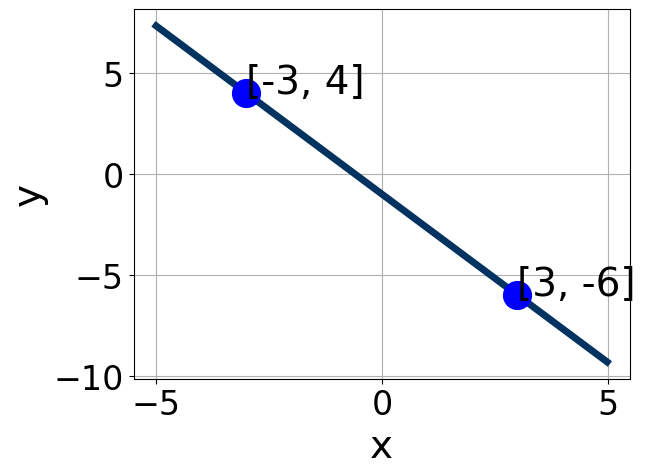
\includegraphics[width=0.5\textwidth]{../Figures/linearGraphToStandardCopyA.png}
\end{center}
\begin{enumerate}[label=\Alph*.]
\item \( A \in [0.7, 3.5], \hspace{3mm} B \in [0.2, 1.18], \text{ and } \hspace{3mm} C \in [-1.09, -0.56] \)
\item \( A \in [0.7, 3.5], \hspace{3mm} B \in [-1.8, -0.81], \text{ and } \hspace{3mm} C \in [0.78, 2.13] \)
\item \( A \in [2.5, 6.3], \hspace{3mm} B \in [-3.1, -2.03], \text{ and } \hspace{3mm} C \in [1.4, 5.33] \)
\item \( A \in [-7.7, -1], \hspace{3mm} B \in [-3.1, -2.03], \text{ and } \hspace{3mm} C \in [1.4, 5.33] \)
\item \( A \in [2.5, 6.3], \hspace{3mm} B \in [2.26, 3.62], \text{ and } \hspace{3mm} C \in [-4.51, -2.8] \)

\end{enumerate} }
\litem{
Write the equation of the line in the graph below in Standard form $Ax+By=C$. Then, choose the intervals that contain $A, B, \text{ and } C$.
\begin{center}
    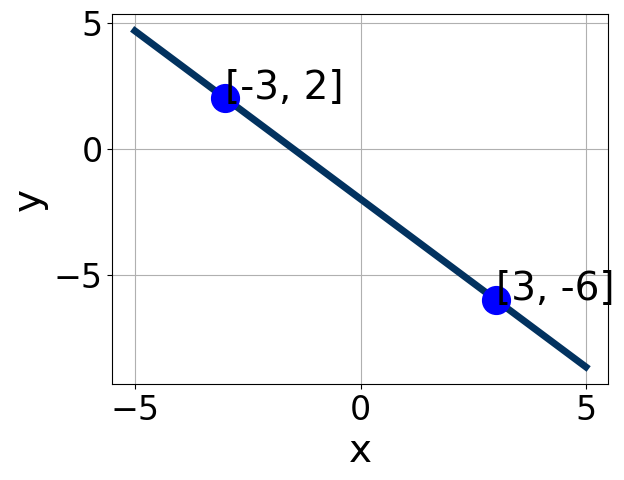
\includegraphics[width=0.5\textwidth]{../Figures/linearGraphToStandardA.png}
\end{center}
\begin{enumerate}[label=\Alph*.]
\item \( A \in [2.4, 5.9], \hspace{3mm} B \in [-6.3, -2.1], \text{ and } \hspace{3mm} C \in [-14, -8] \)
\item \( A \in [-1.3, 2.7], \hspace{3mm} B \in [-2.4, -0.9], \text{ and } \hspace{3mm} C \in [-5, 1] \)
\item \( A \in [-1.3, 2.7], \hspace{3mm} B \in [-0.6, 3.2], \text{ and } \hspace{3mm} C \in [1, 5] \)
\item \( A \in [-4.1, -1.6], \hspace{3mm} B \in [-6.3, -2.1], \text{ and } \hspace{3mm} C \in [-14, -8] \)
\item \( A \in [2.4, 5.9], \hspace{3mm} B \in [3.1, 4.2], \text{ and } \hspace{3mm} C \in [10, 18] \)

\end{enumerate} }
\litem{
Solve the equation below. Then, choose the interval that contains the solution.\[ -7(-19x -10) = -12(4x -15) \]\begin{enumerate}[label=\Alph*.]
\item \( x \in [-2.1, -0.5] \)
\item \( x \in [1.1, 3.1] \)
\item \( x \in [-3.1, -2.5] \)
\item \( x \in [-0.1, 1.2] \)
\item \( \text{There are no real solutions.} \)

\end{enumerate} }
\litem{
Find the equation of the line described below. Write the linear equation as $ y=mx+b $ and choose the intervals that contain $m$ and $b$.\[ \text{Perpendicular to } 8 x + 5 y = 5 \text{ and passing through the point } (5, 6). \]\begin{enumerate}[label=\Alph*.]
\item \( m \in [-0.37, 0.9] \hspace*{3mm} b \in [1.2, 4] \)
\item \( m \in [-1.84, -0.28] \hspace*{3mm} b \in [7.5, 11.1] \)
\item \( m \in [-0.37, 0.9] \hspace*{3mm} b \in [-0.5, 1.7] \)
\item \( m \in [1.32, 1.91] \hspace*{3mm} b \in [1.2, 4] \)
\item \( m \in [-0.37, 0.9] \hspace*{3mm} b \in [-3, -2.3] \)

\end{enumerate} }
\litem{
Solve the linear equation below. Then, choose the interval that contains the solution.\[ \frac{5x + 8}{2} - \frac{5x + 7}{7} = \frac{5x + 8}{4} \]\begin{enumerate}[label=\Alph*.]
\item \( x \in [-2.2, -1.5] \)
\item \( x \in [12.3, 14.6] \)
\item \( x \in [-6, -4.8] \)
\item \( x \in [-0.1, 0.4] \)
\item \( \text{There are no real solutions.} \)

\end{enumerate} }
\end{enumerate}

\end{document}